\section{Causal interventions in model computation}\label{sec:C25:interventions}
Activation inspection begins by recording internal states associated with particular inputs and outputs. A probe can predict a property from an activation without showing that the model uses that property to decide. Correlation can arise because the activation reflects another variable or because the probe extracts information unavailable to the model's downstream computation. Causal claims require interventions and carefully stated counterfactuals.

Activation patching typically compares a clean input, a corrupted input, and a corrupted computation in which selected activations are restored from the clean run. The measured recovery depends on what was corrupted, which sites were patched, and which output metric was used. A patch can have a large effect because it repairs many entangled variables rather than a uniquely interpretable concept. The intervention distribution is therefore part of the claim.

As a methodological foundation, Meng and colleagues' 2022 work uses causal tracing to investigate factual associations and test rank-one model editing through ROME~\cite{meng2022rome}. The important evidence connects localized interventions to measured changes in factual predictions and editing behavior. It does not establish that every fact occupies one isolated location or that editing a weight removes all related knowledge. The result is bounded by model family, prompts, corruption procedure, and evaluation of specificity and generalization.

Zhang and Nanda's 2023 methodological study shows that activation-patching conclusions can change with metrics and corruption methods~\cite{zhang2023patching}. This is a methodological constraint on interpretation: a heatmap is not a mechanism by itself. A convincing study repeats the analysis under justified alternatives, includes negative controls, and reports which conclusions remain stable. If localization shifts dramatically, the appropriate conclusion is sensitivity to the intervention setup, not a precise biological analogy.

The implementation ledger should identify the activation hooks, cached tensors, patch function, corrupted-input constructor, and metric computation. Verify tensor shapes and token positions; a shifted position can patch the wrong event while producing plausible visual output. Then compare no-patch, random-site patch, targeted patch, and relevant ablations. Model outputs should be evaluated on held-out prompts, including cases where the proposed concept is absent or ambiguous. These controls constrain causal interpretation without pretending to reveal the entire model.

The 2026 Certified Interventional Fidelity framework makes adaptive sampling another explicit boundary~\cite{cumulative_c_cif2026}. For a fixed bounded score $Y(x,i)\in[0,1]$, declare input and target-intervention laws $\mathcal D$ and $\Pi$:
\begin{equation}
 \vartheta=\mathbb E_{\mathcal D\times\Pi}[Y(X,I)],\qquad
 q_t=(1-\eta)\Pi+\eta\widetilde q_t,\quad 0<\eta<1.
\end{equation}
If $X_t$ is a fresh independent draw and $q_t$ is selected from past observations before the current score, the importance weight is
\begin{equation}
 w_t=\frac{\Pi(I_t)}{q_t(I_t)}\leq\frac1{1-\eta},\qquad
 \widehat\vartheta_n=\frac1n\sum_{t=1}^n w_tY(X_t,I_t).
\end{equation}
The mixture retains target support while concentrating some queries on suspected failures. A compatible confidence sequence can accommodate repeated looks; searching many explanations additionally requires multiplicity control. This estimates the declared intervention average. It does not identify a uniquely correct circuit or certify that the score captures mechanistic truth. Clipping an unbounded recovery score changes the estimand and must be disclosed.



The sampling path and the evidence-acquisition path impose different identification conditions (Figure~\ref{fig:C25:overview}).
\begin{figure}[!htbp]
\centering
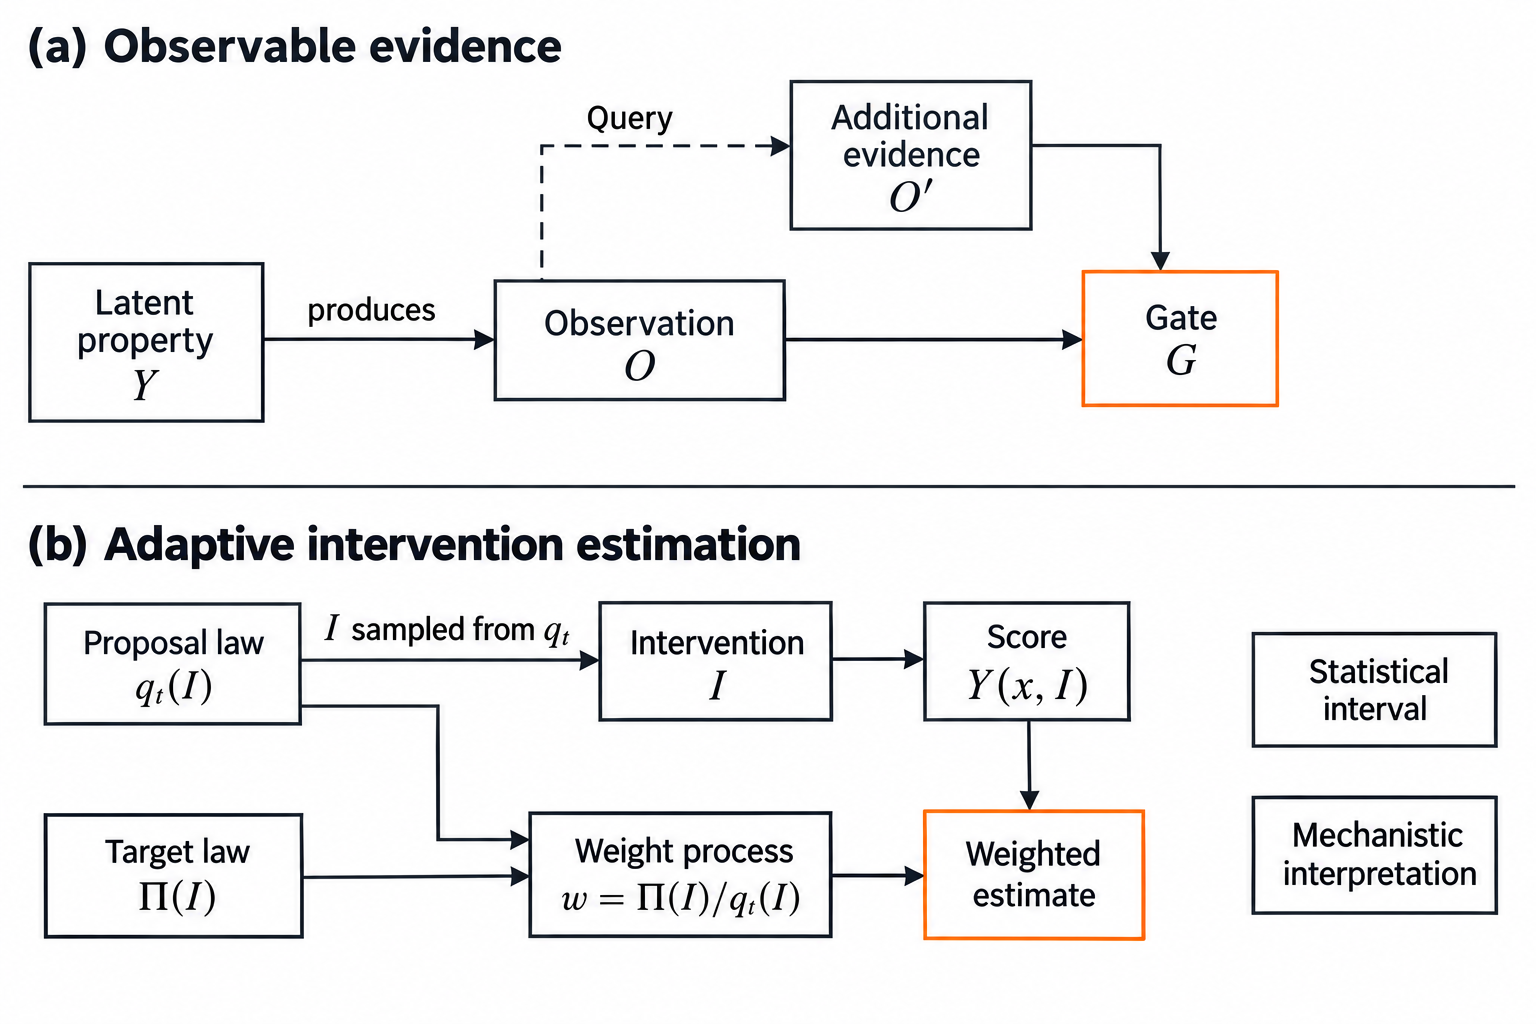
\includegraphics[width=\linewidth]{book/figures/assets/F25review.png}
\caption{Verification depends on evidence and inference. The upper $Y$ is a specified latent property; the lower $Y(x,I)$ is a declared intervention score. Additional queries can change observability. Only $q_t$ samples $I$; both densities are evaluated at that sample to form $w=\Pi(I)/q_t(I)$. Target support and bounded predictable weights are assumptions. An interval for the resulting estimand does not establish mechanistic truth.}
\label{fig:C25:overview}
\end{figure}
